\chapter{関連研究}
\label{chap:system}

この章では人間が文章を読む行為における認知的な動作等の先行研究を示し,
文章表示における読みやすさの指標である視認性に関する研究論文を紹介する.
つづいて,Web上で文章が表示されるにあたって, 活字とは大きく異なるその文体や記法を紹介する.
最後に文章の視認性を操作する既存のライブラリを幾つか紹介する.
これらを踏まえたうえでまとめとして本研究の立ち位置を示す.

\newpage

\section{先行研究}

\subsection{文章の視覚認知に関する研究}
人間の視覚的な情報(光情報)を受容する網膜は中心部分と周辺部分に大別される.
福田(1978)は視覚心理と認知の研究として, 中心部分に映った対象は細かく, 解像度を高く認知でき, 
その一方で周辺部分では視力が低下し, 細やかな文字の識別には中心部の解像力が必要と結論づけた.\cite{福田78} 
ゆえに中心視野よりも大きい幅の文章を読むには眼球運動が行なわれる.
読書運動における眼球運動とは「停留」という単語を注視する状態, 
「サッカード」という次の停留点へと移動するための目の動きが繰り返しであるとされる.以下は神部(1986)が文章中を読むにあたっての
眼球運動にてサッカードと停留を行なった際の注視位置の順番(上)と停留に費やした時間(下)を示した画像である.\cite{神部86}

\begin{figure}[H]
    \centering
    \label{fig:saccade}
    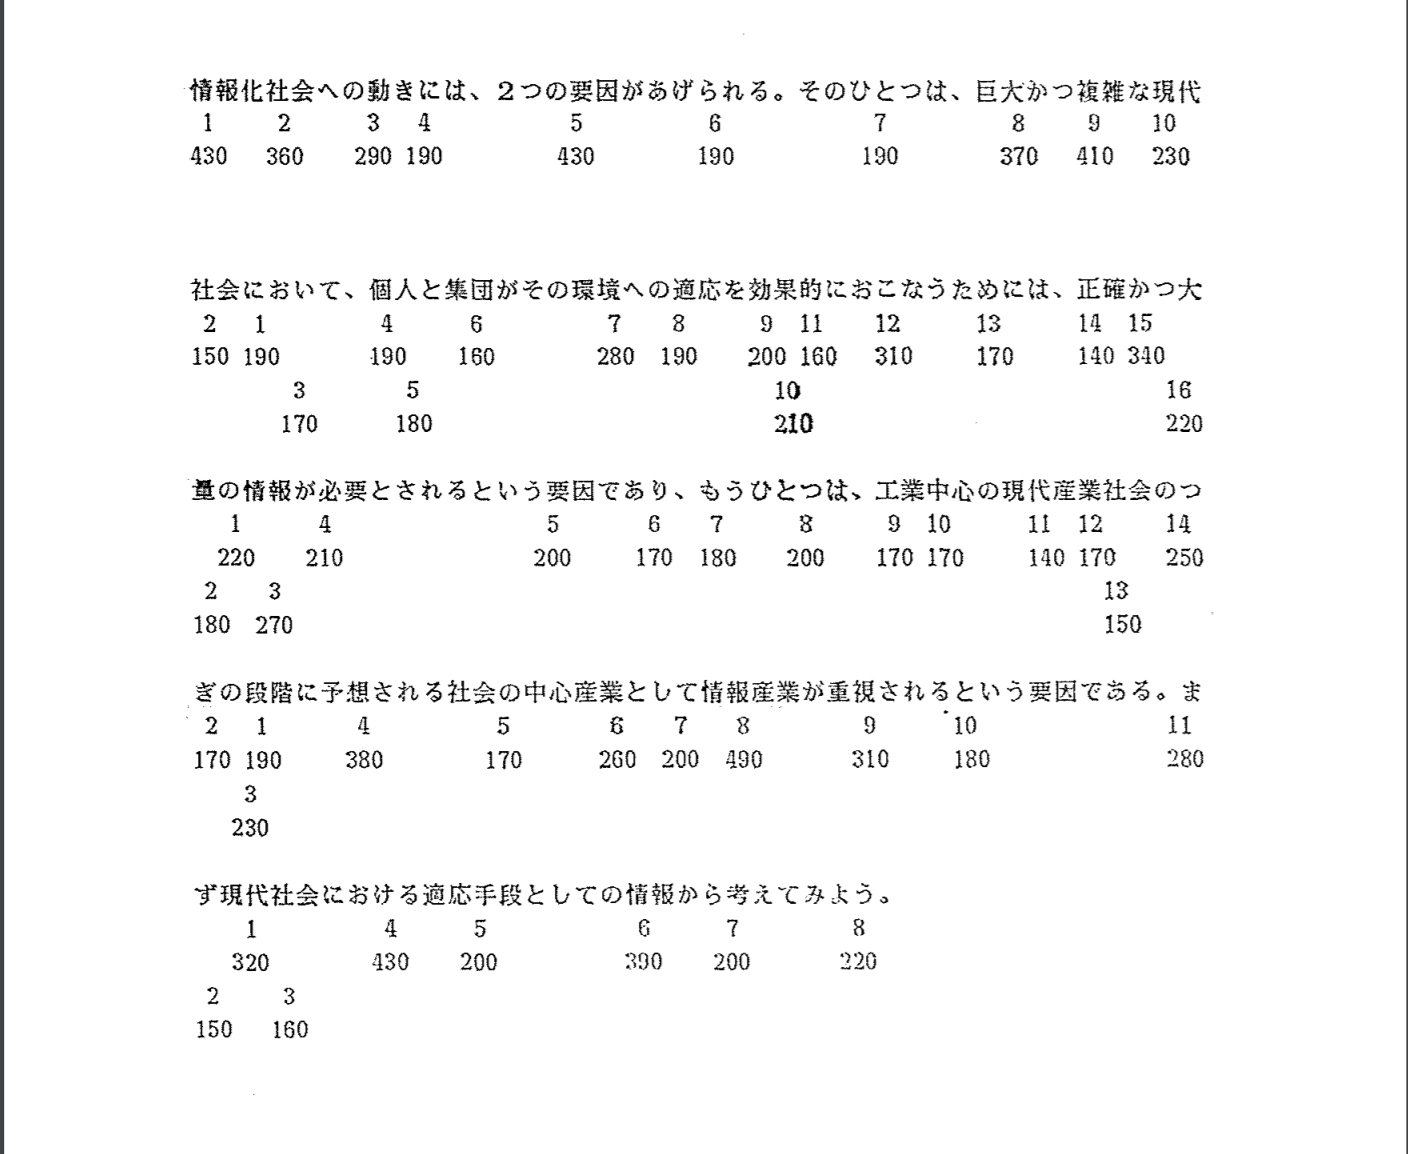
\includegraphics[width=0.6\columnwidth]{image/02/saccade.png}
    \caption[テキスト文の上の注視点の位置と停留時間(msec)の一例]
     {テキスト文の上の注視点の位置と停留時間(msec)の一例 \protect\cite{神部86}より引用}

\end{figure}

これらを踏まえた上で, 神部(1989)は紙媒体での日本語の文章において, 1つの注視点に停留している間に情報が収集される範囲は,
被験者によって個人差があるが,9文字から12文字の範囲であることを明らかにし, 
加えて, 注視点の平均的な文字の移動距離は,3文字から5文字の間とした.\cite{神部89}
また, 中篠(1999)は日本語を読む行為において, 人間の視点移動は文節単位で行われる, と述べた.\cite{中條99} 

\subsection{文章の読みやすさに関する研究}

先ずはじめにリーダビリティ分野の研究には文章の認知のしやすさを指標とする視認性の研究と,
文章の内容自体の分かりやすさを指標とした可読性の研究に大別される.本研究のテーマとして扱っている
文章レイアウトの調整は文章の視認性の分野に属するものとする.これらを踏まえた上で文章の視認性に関連した研究を紹介する.

村田らはリアルタイムでの講演会における登壇者の音声から自動で字幕を生成する際の
視認性を向上させる研究の中で, 話言葉はその意味のまとまりを考慮し改行を行うことにより, 
字幕の視認性が向上したことを報告している.\cite{村田09} 

小林らは, 電子リーダーを用いた読む速さの効率化の研究において, 文章を
折返し箇所にて文節を分断しない改行レイアウトを提案, 
文節を追いやすいレイアウト(以下文節間改行レイアウト)を作成することで視線が停まる回数を減し, 
通常の両端揃えのレイアウトより読み速度が向上すると報告している.\cite{小林14} 

\begin{figure}[H]
    \centering
    \label{fig:layout}
    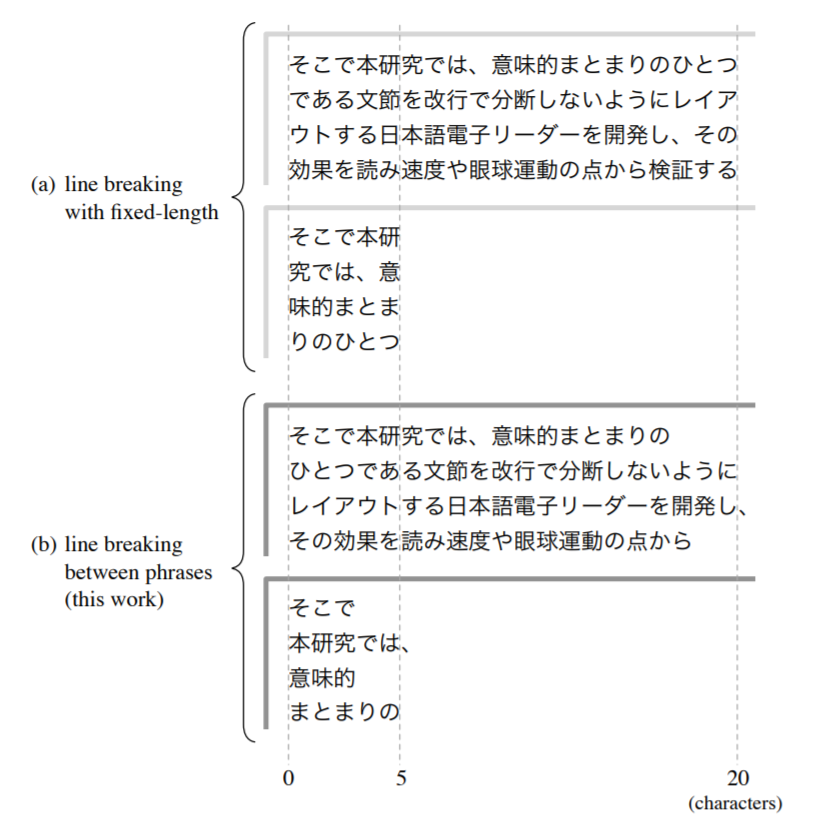
\includegraphics[width=0.6\columnwidth]{image/02/img1.png}
    \caption[文節を分断しない改行レイアウト] {文節を分断しない改行レイアウト\protect\cite{小林14}より引用}
\end{figure}

\section {Web上の文章の特色}
本節では組版ルールに則らない, 紙媒体とは異なったweb上の独自の記法を紹介する.
これは文章レイアウトの視認性を向上させる処理を行うにあたって従来の組版ルールに加えて
文字列以外のデータを取り扱う必要がある,
Webブラウザ上であることを前提として,Web上で書かれる文章はHTMLで書かれており,Webブラウザ上で文章はその文章が格納されたDOMとして解釈される.
日本語の横書きの文章はCSSによるスタイルの設定にも依存するが, 基本そのDOMに規定された範囲内に左詰めで挿入される.

\footnotetext[1]{
    参考: \protect\url{https://twitter.com/yousuck2020/status/1212025675055452160}
}

\subsubsection{URLリンク}

文章内にURLリンクを貼り付けたり, 文字の中にURLリンクを埋め込むことが可能である.
近年ではTwitter, Instagramの投稿においてメタデータタグを \# (ハッシュタグ)といった特定の記号のあとに文章を記述することで
文字列をラベルとしたメタデータを挿入することが可能となる仕様も存在し,広く扱われている.
\begin{figure}[H]
    \centering
    \label{fig:hush}
    
\includegraphics[width=0.6\columnwidth]{image/02/img_3.png}
    \caption[ハッシュタグを用いたメタデータを埋め込んだ投稿の例]{ハッシュタグを用いたメタデータを埋め込んだ投稿の例\footnotemark[1]}
\end{figure}

\footnotetext[2 
]{
    参考: \protect\url{https://twitter.com/yousuck2020/status/1212025675055452160}
}

\subsubsection{emoji}
Emojiとは特定のユニコードを読み込むことで文章中に埋め込むことができるアイコンである.文章を装飾できたり, 
明示的に感情や場所, 季節感を表現できるという利点がある.近年ではスマートフォンやIMEでも簡易的に打ち込むことができるため, 
SNS上や砕けた文体の文章では多用され, 句読点の代用として使用されることもある.
\begin{figure}[H]
    \centering
    \label{fig:emoji}
    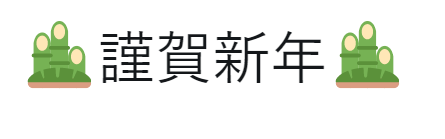
\includegraphics[width=0.6\columnwidth]{image/02/img_1.png}
    \caption[emojiを利用した文章装飾の例]{emojiを利用した文章装飾の例}
\end{figure}

\subsubsection{句点代わりの改行}
日本語組版に基づく方法以外に文章の文意や内容を切り分ける方法として, 改行を入れる手法が散見される.また, 
改行を連続して二度以上いれることで一行以上の余白を作り, 文章の意味段落的に分ける手法も存在する.
後者に関してはスタイルの都合上問題ないと考えられるが,前者に関してはDOMの横幅が大きくとられているゆえ,
一行あたりが長くなることで視認性を損ねてしまうケースを見越し, 書き手側が文章の途中で改行を入れるというパターンが発生する可能性があり, 
前章の研究動機にて述べたWeb上の文章において「書き手と読み手側のレイアウトのズレ」は, この「句点代わりの改行」によって発生するケースで散見される.

\begin{figure}[H]
    \centering
    \label{fig:midashi}
    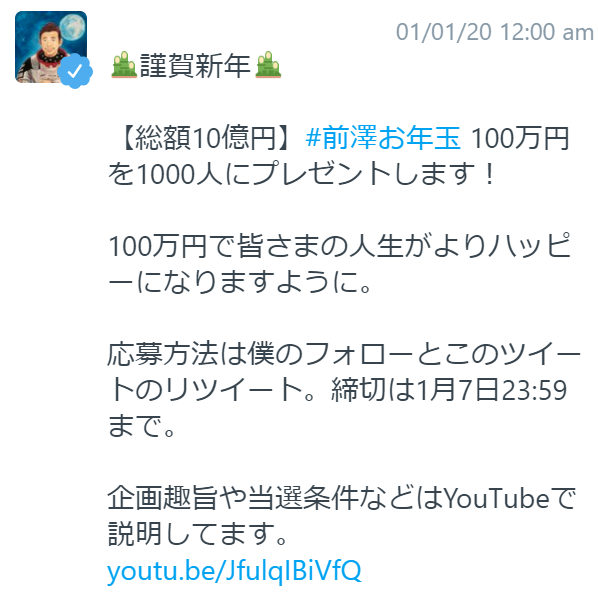
\includegraphics[width=0.6\columnwidth]{image/02/img_4.png}
    \caption[改行により見出しを分けた例] {改行により見出しを分けた例\footnotemark[1]}
\end{figure}

\subsection{ライブラリ}
前節のWeb上のテキストの特色を踏まえた上で, 小林らが開発した文節間改行レイアウトを行う
既存のライブラリとして書き手側で用いる
Budou\footnotemark[2], mikan.js\footnotemark[3],

\footnotetext[2]{
    \protect\url{https://developers-jp.googleblog.com/2016/10/budou.html}
}

\footnotetext[3]{
    \protect\url{https://github.com/trkbt10/mikan.js}
}
\subsubsection{Budou}

BudouはPythonで書かれたGoogle製の形態素解析APIであるCloud Natural Language API
を用いたライブラリであり, テンプレートエンジンのフィルターやビルドツールのタスクとして
エディターに組み込んで利用する.
単語の境界判別と構文解析を行い文節を特定し, 文節ごとに特定のHTML要素を囲むことで, 
文節ごとに文章を分離, 改行を加えることができる.
利用するにあたってのデメリットはAPIをたたくため,その設定や通信が必要であるがゆえに
ローカル環境で完結しない点と, そのリクエストが多くなると料金が発生する点にある.
また, 見出し語で用いることを前提としているため, 長文で行うことが困難である.

\begin{figure}[H]
    \centering
    \label{fig:image7}
    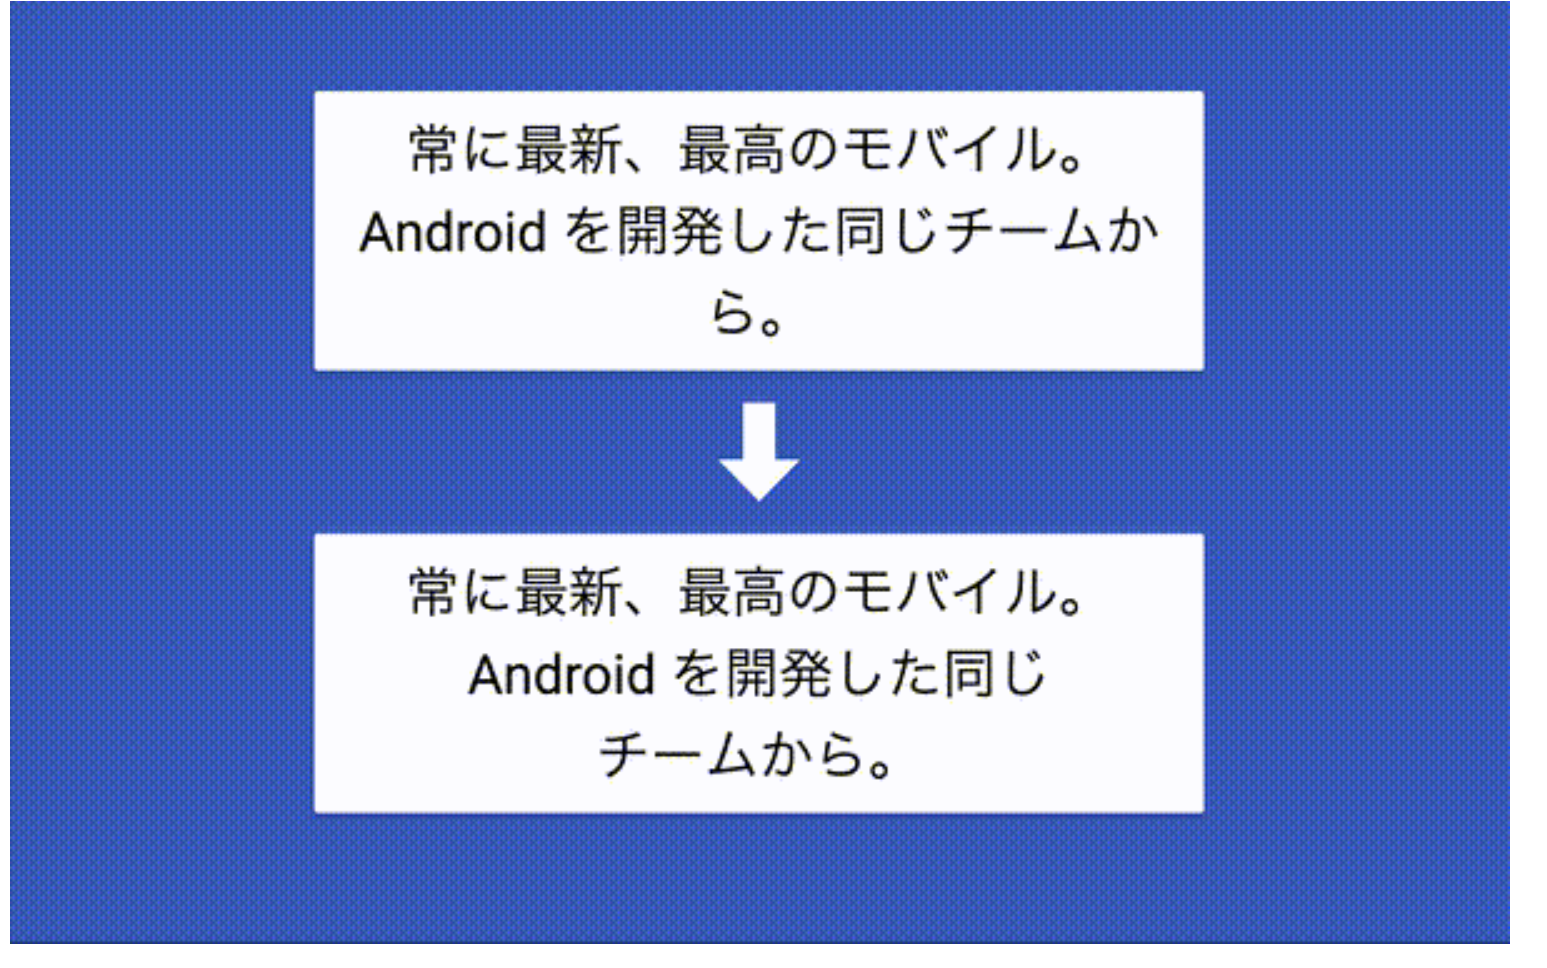
\includegraphics[width=0.6\columnwidth]{image/02/img2.png}
    \caption[Budouの動作イメージ] {Budouの動作イメージ\footnotemark[3]}
\end{figure}

\subsubsection{mikan.js}

mikan.jsは先述したBudouの問題点を解決するべくtrkbt10氏が開発したJavaScriptライブラリである.
簡易的な正規表現を用いて文の区切れを特定し, Budouと同じ仕組みで改行を加えている.
当ライブラリの利点はJavaScript製であるためWebサイトに導入しやすく,汎用性が高い点にある.
一方のデメリットとして,簡易的な正規表現を利用したことにより, 
大雑把な単位で文章を区切るため文章のレイアウトが損ねる点にある.またURLリンクや記号といった日本語以外の
文章に対しては精度が低いこともあげられる.また, Budouと同じ仕組みで改行を行うため, 
同じく短文や見出し語といった限られた範囲での利用のみが想定されている.

\begin{figure}[H]
    \centering
    \label{fig:image8}
    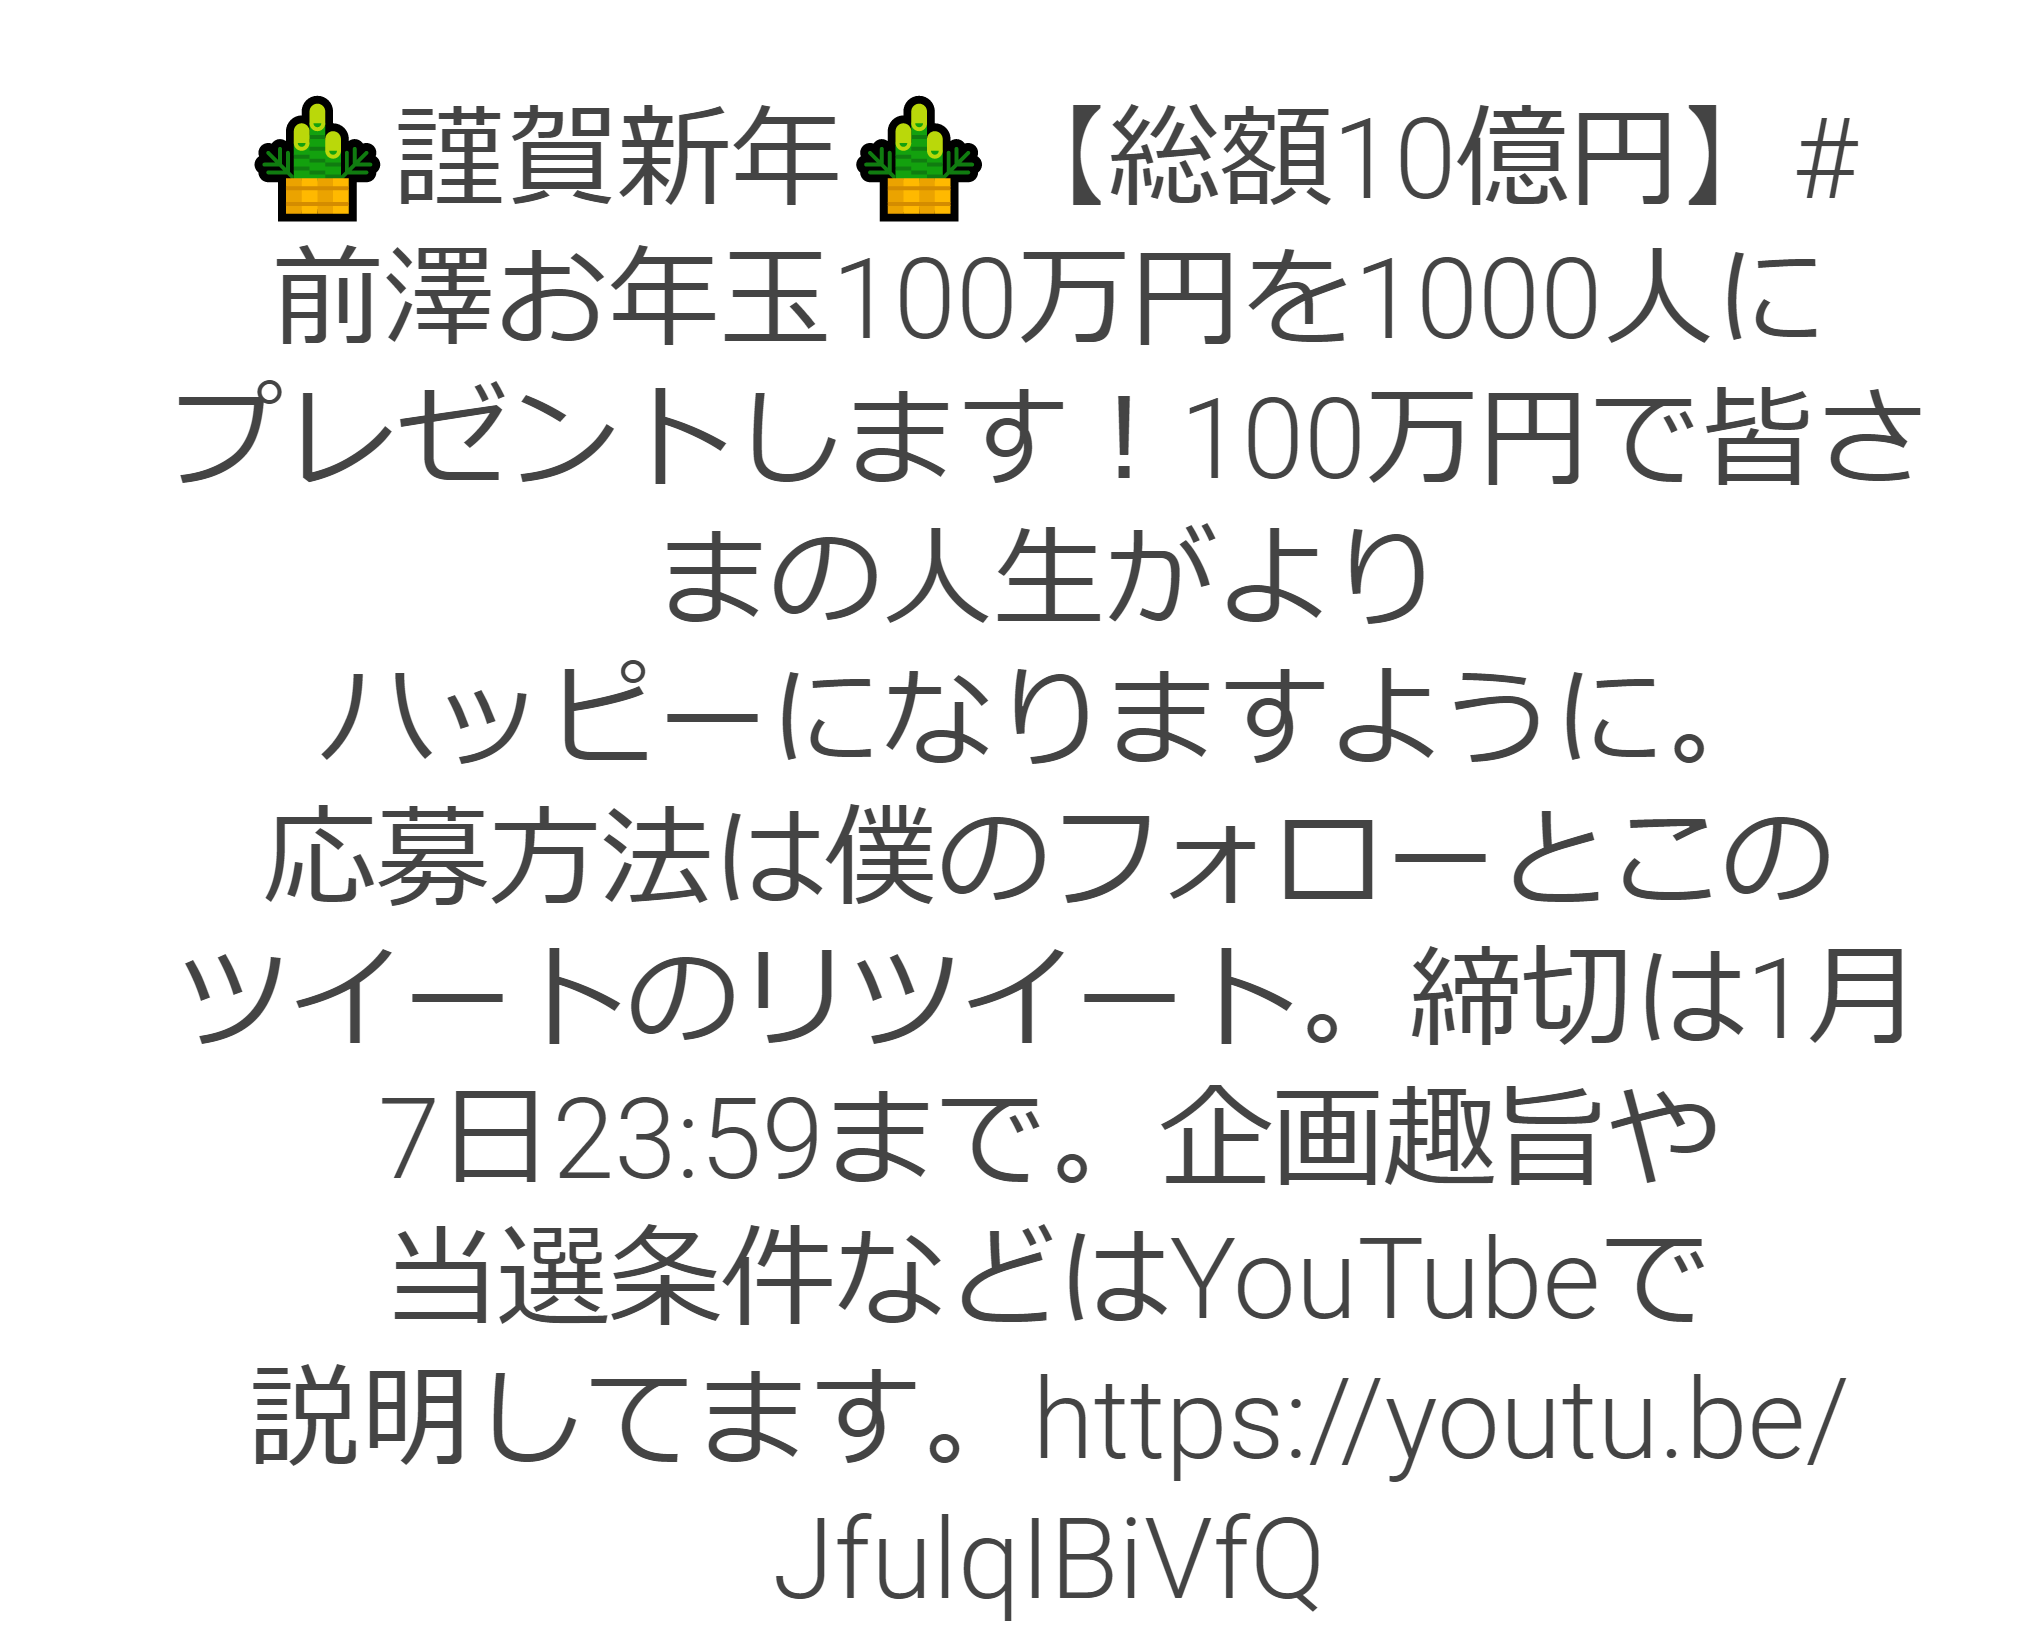
\includegraphics[width=0.6\columnwidth]{image/02/img3.png}
    \caption[mikan.jsのデモ画面にて記号やURLを表示した例]{mikan.jsのデモ画面にて記号やURLを表示した例\footnotemark[4]}
\end{figure}

ここで双方に共通する特色として, 先述したように見出し語といった短い文章を想定している点, 
あくまでHTMLで文章を書く際に, 文章の改行位置を自動的に選定するために用いるライブラリである点
が挙げられる.
%なぞ
前者に関しては文章内容の視認性については処理を苦手としており, 後者に関しては
書き手側がSNSやブログのエディター画面では用いることを想定しており, 
書き手側の不満を解消しているライブラリだと言える.

\subsection{拡張機能}
読み手が読む文章の視認性上げる拡張機能としてEasyReaderを紹介し, その特色を述べる. \footnotemark[4]
\subsubsection{EasyReader}

\footnotetext[4]{
    \protect\url{https://chrome.google.com/webstore/detail/easyreader/boamfheepdiallipiieadpmnklbhadhc}
}

EasyReaderはGoogle Chromeのブラウザ拡張として配布されているサードパーティライブラリであり,閲覧しているWebページのテキストを選択した後に
その文章のユーザーが指定したフォント設定,フォントサイズに変更したものをモーダルページ上に新たに表示する, というアプリケーションである.
このアプリの利点は既存の文章をユーザー個人の設定に基づいた表示を行うことで,視認性を向上できるという点である.

\begin{figure}[H]
    \centering
    \label{fig:image_5}
    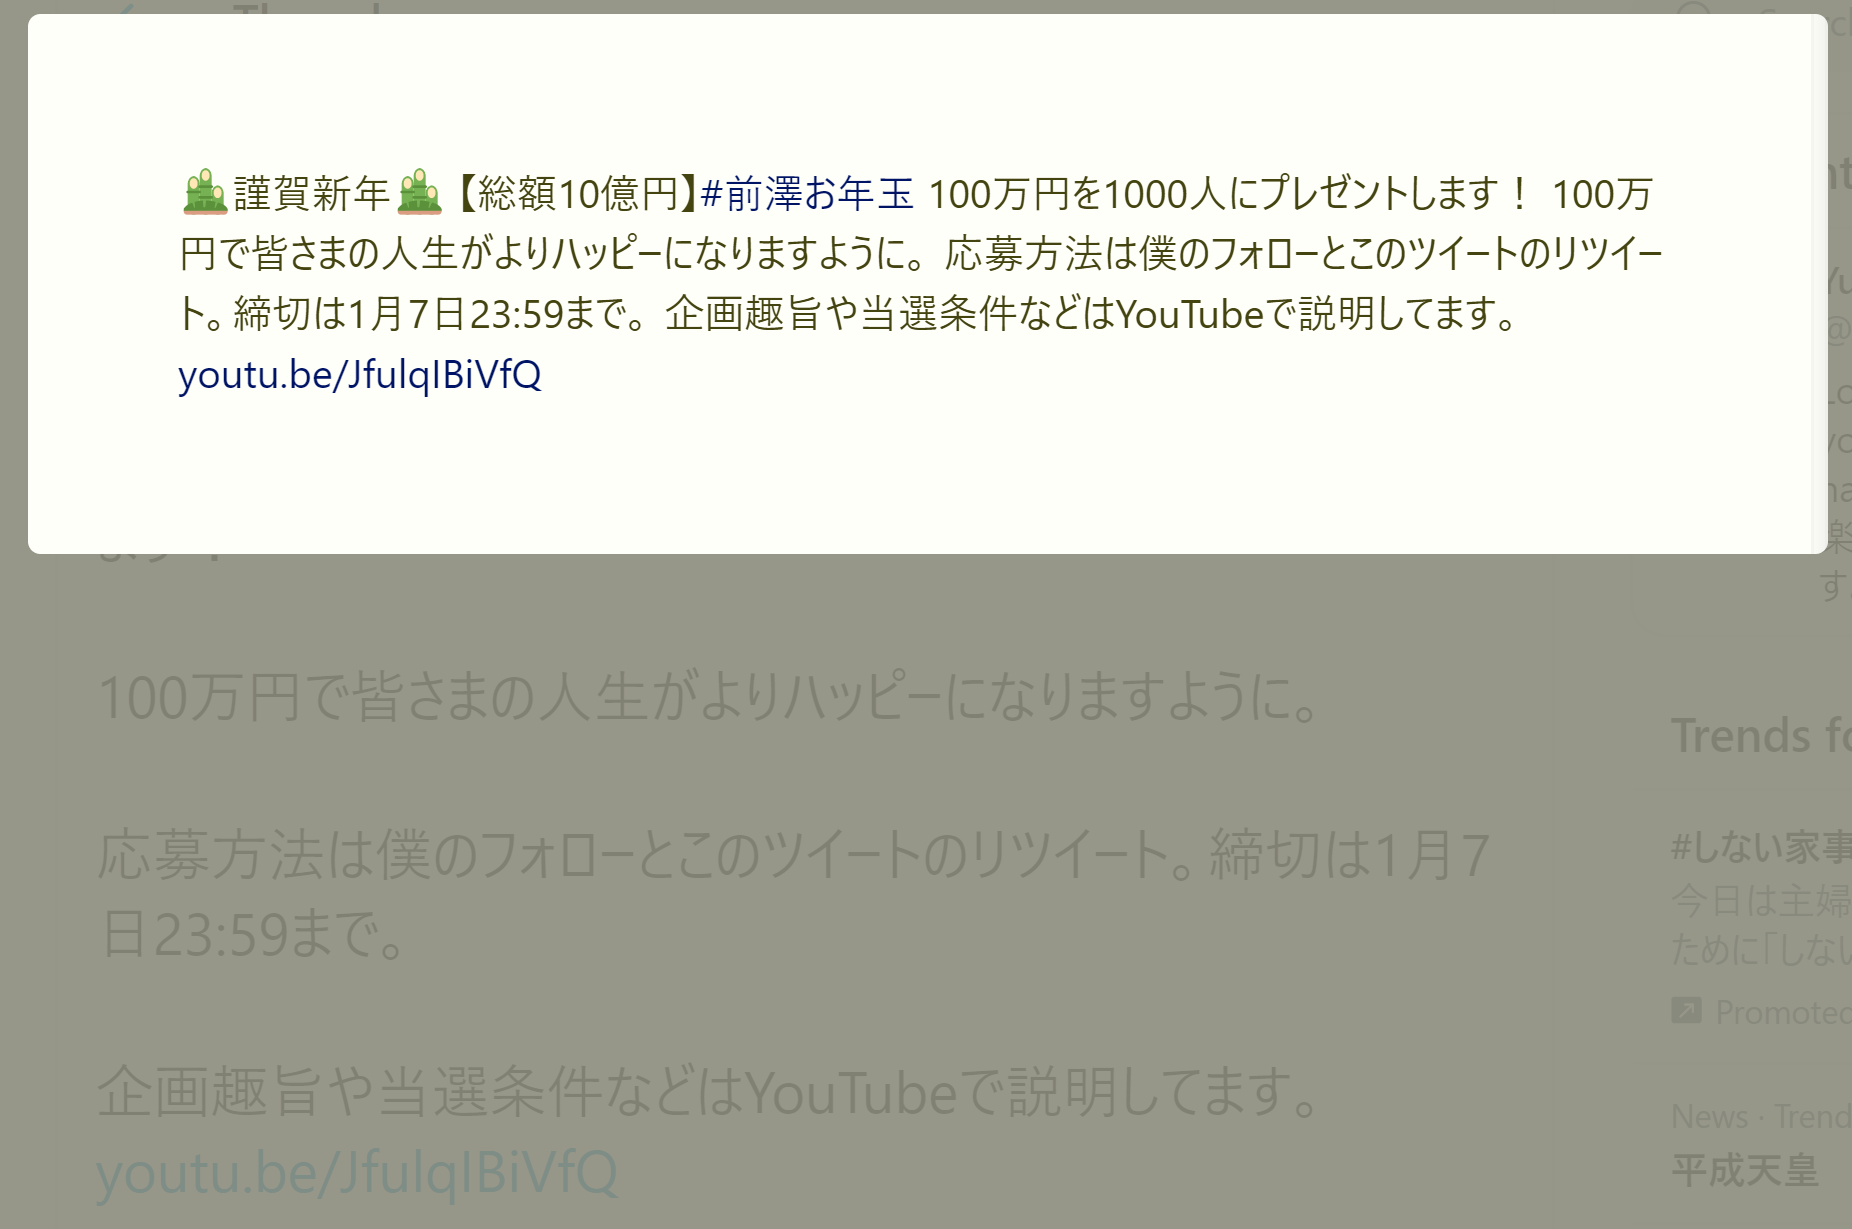
\includegraphics[width=0.6\columnwidth]{image/02/img_5.png}
    \caption[EasyReaderを用いた例]{EasyReaderを用いた例}
\end{figure}

以上のようなライブラリ,及び拡張ツールが存在した
一方,読み手側の環境であらかじめ崩れていた文章レイアウトを表示していた状態で,その文章レイアウトの改稿を行うことを主としたライブラリ,および拡張機能は見当たらなかった.

\section{まとめ}
まず, 人間の視覚認知の研究から人が文章を読む際に行う行動について紹介した.
その上で文章の読む文章のリーダビリティの研究は視認性と可読性の二種類に大別され, 
文章レイアウトの改稿は前者の分野に属することを述べた.
そして, 本研究では文章のレイアウトを変更する, という視認性の操作を行い
可読性には関与しないものとして取り扱うこととした.
また, 小林ら文章の視認性をあげる方法として, 文節間の区切りを改行箇所として区切り,
表示する研究を紹介し, その有意性を示した.
続いてWeb上には組版ルールに縛られない,さまざまな文字装飾や記法が存在するとして, それらが
書き手側に1つの記法として浸透していることを示した.
つづいて,Budou, mikan.jsといった文節間改行レイアウトを実現できるライブラリを紹介し, 
それらの問題点として書き手側が文章を打ち込むエディターなどに前もってライブラリを入れる, 
または文章の記述途中の段階でライブラリを組み込む必要がある点と長文には不向きな設計であることを述べた.
また,読み手側が文章を読みやすいスタイルに変更した上で提示するライブラリは配布されているが,
読み手側の環境では視認性を損ねている場合, 読み手側自身のデバイスで自動的に視認性の高いレイアウトに変更する
ライブラリ,拡張機能の存在は散見されなかった.

本研究では, 読者の文章レイアウトに着目し, 読者側の操作で閲覧環境に則り,
視認性の高い文章レイアウトを再形成することを支援するアプローチをとる実装を行う.